% ------------------------------------------------------------------------
% ------------------------------------------------------------------------
% ICMC: Modelo de Trabalho Acadêmico (tese de doutorado, dissertação de
% mestrado e trabalhos monográficos em geral) em conformidade com 
% ABNT NBR 14724:2011: Informação e documentação - Trabalhos acadêmicos -
% Apresentação
% ------------------------------------------------------------------------
% ------------------------------------------------------------------------

% Opções: 
%   Qualificação          = qualificacao 
%   Curso                 = doutorado/mestrado
%   Situação do trabalho  = pre-defesa/pos-defesa (exceto para qualificação)
%   Versão para impressão = impressao
\documentclass[mestrado, pre-defesa]{packages/icmc}

% ---------------------------------------------------------------------------
% Pacotes Opcionais
% ---------------------------------------------------------------------------
\usepackage{rotating}           % Usado para rotacionar o texto
\usepackage[all,knot,arc,import,poly]{xy}   % Pacote para desenhos gráficos
% Este pacote pode conflitar com outros pacotes gráficos como o ``pictex''
% Então é necessário usar apenas um dos pacotes conflitantes
\newcommand{\VerbL}{0.52\textwidth}
\newcommand{\LatL}{0.42\textwidth}
\newcommand{\figref}[1]{\figurename~\ref{#1}}
% ---------------------------------------------------------------------------


% ---
% Informações de dados para CAPA e FOLHA DE ROSTO
% ---
% Tanto na capa quanto nas folhas de rosto apenas a primeira letra da primeira palavra (ou nomes próprios) devem estar em letra maiúscula, todas as demais devem ser em letra minúscula.
\tituloPT{Animação de fumaça em malhas não-estruturadas usando RBF-FD}
\tituloEN{Smoke animation on unstructured meshes using RBF-FD}
\autor[da Silva, G. L.]{Gabriel Lucas da Silva}
\genero{M} % Gênero do autor (M = Masculino / F = Feminino)
\orientador[Orientador]{Prof. Dr.}{Afonso Paiva Neto}
%\coorientador{Prof. Dr.}{Fulano de Tal}
\curso{CCMC}
\data{19}{08}{2025} % Data do depósito
\idioma{PT} % Idioma principal do documento (PT = português / EN = inglês)
% ---


% ---
% RESUMOS
% ---

% Resumo em PORTUGUÊS
% conter no máximo 500 palavras
% conter no mínimo 1 e no máximo 5 palavras-chave
\textoresumo[brazil]{
    Durante as últimas décadas, os estudos de simulações numéricas de escoamento de fluidos e de novas técnicas de processamento geométrico têm sido áreas de intensa pesquisa e com aplicações que vão da engenharia industrial à indústria do entretenimento. Nesse projeto de mestrado, propomos o estudo de novas técnicas de animação de escoamento de fumaça em domínios arbitrários usando interpolações que não necessitam de malha. Essas técnicas consistem na aplicação do método numérico sem malha conhecido como RBF (Radial Basis Function) e sua versão com diferenças finitas generalizadas (RBF-FD).
    }{RBF-FD, Animação de fumaça, Malhas não-estruturada, Domínios arbitrários}


% resumo em INGLÊS
% conter no máximo 500 palavras
% conter no mínimo 1 e no máximo 5 palavras-chave
\textoresumo[english]{
    Over the last decades, studies of numerical simulations of fluid flow and new geometric processing techniques have been areas of intense research with applications ranging from industrial engineering to the entertainment industry. In this master's project, we propose the study of new smoke flow animation techniques in arbitrary domains using mesh-free interpolations. These techniques consist of applying the meshless numerical method known as RBF (Radial Basis Function) and its version with generalized finite differences (RBF-FD).
    }{RBF-FD, Smoke animation, Unstructured mesh, Arbitrary domains}


% ----------------------------------------------------------
% ELEMENTOS PRÉ-TEXTUAIS
% ----------------------------------------------------------

% Inserir a ficha catalográfica
\incluifichacatalografica{tex/pre-textual/ficha-catalografica.pdf}

% DEDICATÓRIA / AGRADECIMENTO / EPÍGRAFE
\textoagradecimentos*{tex/pre-textual/agradecimentos}

% Inclui a lista de figuras
\incluilistadefiguras

% Inclui a lista de tabelas
\incluilistadetabelas

% ----
% Início do documento
% ----
\begin{document}
% ----------------------------------------------------------
% ELEMENTOS TEXTUAIS
% ----------------------------------------------------------
\textual
\chapter{Introdução}
\label{chapter:introducao}

\begin{figure}
    \centering
    \includegraphics[width=0.92\textwidth]{images/mass_effect3_smoke.jpg}
    \caption{Animação de fumaça no jogo \textit{Mass Effect 3}.}
    \subcaption*{Fonte: \url{https://www.fxguide.com/fxfeatured/cinematics-case-study-mass-effect-3/}}
    \label{fig:masseffect3}
\end{figure}

As indústrias do entretenimento, jogos (\figref{fig:masseffect3}) e engenharia têm grande interesse em simulações de fluidos para integrar em seus respectivos produtos. Em geral, simulações baseadas em física tendem a apresentar resultados visualmente realísticos e convincentes, podendo levar uma pessoa leiga na área a confundir uma gravação real com uma simulação \cite{Huang2015}. É necessário que o observador da simulação seja convencido da sua veracidade, pois isso aumenta a imersão na experiência de um filme ou jogo. Para alcançar esse nível de qualidade desejado, é preciso trabalhar com técnicas computacionalmente custosas, para perder o mínimo de detalhes possível na simulação. Portanto, é importante utilizar métodos com alta precisão e otimização do tempo de execução, para poder aplicar a técnica em tempo real, no caso de jogos, e poupar tempo na produção de efeitos especiais em filmes.

O comportamento de fluidos no mundo real é descrito de maneira contínua. Quando se discretiza este fenômeno para simular computacionalmente, é necessário realizar um passo de discretização do domínio. Por conta disto, simulações de fluidos podem ser abordadas de duas maneiras mais comumente usadas: visão lagrangiana e visão euleriana, além da forma híbrida.

Na visão lagrangiana (ver \figref{fig:lagrangiana}), o fluido é discretizado em forma de um sistema de partículas, com cada uma delas representando uma parte da massa fluídica (volume). Cada partícula tem uma posição no domínio e carrega consigo algumas propriedades daquela parte do fluido que a mesma está discretizando, como velocidade, posição, pressão e força externa. A simulação é realizada pela determinação, em cada passo de tempo, da posição e velocidade de cada partícula do sistema. Já na abordagem euleriana (ver \figref{fig:euleriana}), a discretização do espaço é feita em uma grade ou malha. Esta grade é dividida em células, e estas armazenam as propriedades do fluido que estão passando por aquela região do espaço, sendo responsáveis por gerir como o fluido irá escoar.

\begin{figure}
    \centering
    \caption{Tipos de simulações de escoamento de fluidos}
    \begin{subfigure}[b]{0.45\textwidth}
        \centering
        \includegraphics[width=\textwidth]{images/lagrangeana.pdf}
        \caption{Simulação pela visão lagrangiana.}
        \label{fig:lagrangiana}
    \end{subfigure}
    \hfill
    \begin{subfigure}[b]{0.45\textwidth}
        \centering
        \includegraphics[width=\textwidth]{images/euleriana.pdf}
        \caption{Simulação pela visão euleriana.}
        \label{fig:euleriana}
    \end{subfigure}
    \subcaption*{Fonte: Elaborada pelo autor.}
    \label{fig:simulacoes}
\end{figure}

Existem diversas características que diferem na representação da malha. Por exemplo, existem malhas regulares e irregulares. Em malhas regulares, os centros de cada célula são equidistantes e colineares, enquanto nas malhas irregulares não existe esta restrição. Outro fator que pode distinguir é a topologia de cada célula da malha: existem malhas com topologia tetraédrica, hexaédrica ou mistas. Malhas tetraedrais se moldam melhor em fronteiras irregulares, como objetos complexos, porém, este benefício é contrabalançado pelo grande custo computacional. Malhas hexaédricas têm a desvantagem de perder muitos detalhes por conta da estrutura simples. Grades híbridas têm a vantagem de poder usar células tetraédricas em fronteiras com objetos complexos, e células hexaédricas em espaços abertos, melhorando o custo computacional \cite{Huang2015}. Além disso, os valores do campo escalar ou campo vetorial podem ser armazenados no centro de cada célula ou no centro de cada face. Caso ambos estejam no centro, esta malha é chamada de co-localizada (do inglês, \textit{collocated}), e no caso do campo escalar estar no centro da célula e a velocidade na face, esta malha é chamada de deslocada (do inglês, \textit{staggered}), conforme ilustrado na \figref{fig:celulas}. O foco do nosso trabalho será a simulação de fluidos por meio da abordagem euleriana com uso de malhas tetraedrais deslocadas.

\begin{figure}
    \centering
    \caption{Tipos de células presentes na abordagem euleriana em duas dimensões.}
    \begin{subfigure}[b]{0.23\textwidth}
        \centering
        \includegraphics[width=\textwidth]{images/quad_collocated.pdf}
        \caption{Célula quadricular co-localizada.}
        \label{fig:quadcollo}
    \end{subfigure}
    \hspace{0.1\textwidth}
    \begin{subfigure}[b]{0.23\textwidth}
        \centering
        \includegraphics[width=\textwidth]{images/quad_staggered.pdf}
        \caption{Célula quadricular deslocada.}
        \label{fig:quadstagg}
    \end{subfigure}
    \newline
    \begin{subfigure}[b]{0.23\textwidth}
        \centering
        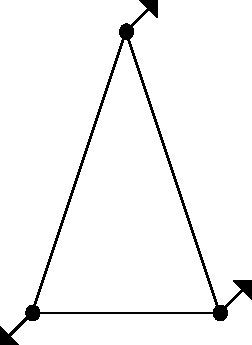
\includegraphics[width=\textwidth]{images/tri_collocated.pdf}
        \caption{Célula triangular co-localizada.}
        \label{fig:tricollo}
    \end{subfigure}
    \hspace{0.1\textwidth}
    \begin{subfigure}[b]{0.23\textwidth}
        \centering
        \includegraphics[width=\textwidth]{images/tri_staggered.pdf}
        \caption{Célula triangular deslocada.}
        \label{fig:tristagg}
    \end{subfigure}
    \subcaption*{Fonte: Elaborada pelo autor.}
    \label{fig:celulas}
\end{figure}

Em geral, simulações de fluidos baseadas em física têm como base as Equações de Navier-Stokes (ENS) para fluidos incompressíveis \cite{incompressible}. Estas são um conjunto de equações diferenciais parciais que descrevem o escoamento dos fluidos. Para resolver as ENS, é necessária a aplicação de operadores diferenciais de cálculo vetorial, tais como: gradiente, divergente e laplaciano. Estes operadores são aplicados em funções contínuas; no entanto, não é possível representar funções contínuas em computadores, logo, estas devem ser discretizadas. Na abordagem euleriana, o método de Diferenças Finitas (do inglês, \textit{Finite Differences} - FD) visa solucionar este problema para grades uniformes. A aplicação de FD em uma célula da grade necessita acessar informações dos vizinhos; estes vizinhos são chamados de estêncil, no caso 2D são 4 e no 3D são 6, conforme mostrado na \figref{fig:stencils}. Como esta vizinhança é fixa em grades uniformes, podemos aplicar este método de forma eficiente.

\begin{figure}
    \centering
    \caption{Tipos de estênceis em grades uniformes.}
    \begin{subfigure}[b]{0.23\textwidth}
        \centering
        \includegraphics[width=\textwidth]{images/stencil-2d.pdf}
        \caption{Estêncil 2D.}
        \label{fig:2dsten}
    \end{subfigure}
    \hspace{0.1\textwidth}
    \begin{subfigure}[b]{0.23\textwidth}
        \centering
        \includegraphics[width=\textwidth]{images/stencil-3d.pdf}
        \caption{Estêncil 3D.}
        \label{fig:3dsten}
    \end{subfigure}
    \subcaption*{Fonte: Elaborada pelo autor.}
    \label{fig:stencils}
\end{figure}

Quando trabalhamos com malhas tetraedrais, temos que aceitar uma malha não-estruturada. Esta propriedade impossibilita o uso de FD, pois a vizinhança de uma célula não é fixa, sendo necessário o uso de outros métodos para a resolução destes operadores diferenciais em malhas não-estruturadas, tais como os métodos de Elementos Finitos e Volumes Finitos. Em animação computacional, o método de Volumes Finitos (do inglês, \textit{Finite Volumes} - FV) é o mais utilizado para animação de fumaça em malhas não-estruturadas \cite{Klingner2006}.

Outra propriedade importante de malhas que deve ser considerada é a conformidade, que consiste na topologia da mesma. Uma malha conforme (ver \figref{fig:conforme}) contém todas as arestas da face completa, ou seja, não existe um vértice que resida no interior de uma aresta. Na literatura, encontramos diversos problemas geométricos \cite{Mahmood2019, nonconf1} em malhas não-conformes (ver \figref{fig:africa}). No entanto, há uma lacuna na resolução das ENS nesse tipo de malha. Para resolver numericamente as ENS, é interessante utilizar um método que seja independente da malha, isto é, métodos de interpolação sem malha.

\begin{figure}
    \centering
    \caption{Exemplo de malha conforme.}
    \includegraphics[width=0.7\textwidth]{images/africa-conforme.jpg}
    \subcaption*{Fonte: \cite{Nascimento:2014}}
    \label{fig:conforme}
    \vspace{-1.2cm}
\end{figure}

\begin{figure}
    \centering
    \caption{Exemplo de malha não-conforme, com círculo vermelho para evidenciar uma aresta que mostra a propriedade da malha.}
    \includegraphics[width=0.7\textwidth]{images/africa-nao-conforme.png}
    \subcaption*{Fonte: Adaptado de \cite{Nascimento:2014}}
    \label{fig:africa}
\end{figure}

O método baseado em Funções de Base Radial (do inglês, \textit{Radial Basis Function} - RBF) \cite{rbf} faz uma interpolação independente de malha, e sua aproximação de FD conhecida como \textit{Radial Basis Function Finite Differences} (RBF-FD) \cite{WRIGHT200699}, resolve os operadores diferenciais necessários. Logo, com a aplicação do RBF-FD em malhas não-conformes, pretendemos resolver as ENS e representar visualmente a simulação da fumaça.

\section{Objetivos}

O objetivo principal deste trabalho é desenvolver uma técnica eficiente de animação de fumaça em malhas não-estruturadas utilizando o método RBF-FD, abordando as limitações atuais na aplicação de condições de contorno em malhas tetraedrais.


\section{Roteiro}

O resto do texto se divide da seguinte maneira. No capítulo \ref{chapter:revisao}, abordaremos como evoluiu a simulação de fluidos computacional ao longo do tempo, avaliando os métodos canônicos até os métodos mais atuais. No capítulo \ref{chapter:fundteorica} demonstraremos a fundamentação teórica que basea nossa solução e enunciar os problemas a serem resolvidos. No capítulo \ref{chapter:metodologia}, explicaremos os principais métodos utilizados na nossa pesquisa, como o RBF-FD, e como aplicar as condições de contorno de Neumann neste caso. Por fim, No capítulo \ref{chapter:Resultados}, daremos um contexto geral do nosso projeto, explicitando as expectativas, hipóteses e o cronograma para o desenvolvimento do projeto.


\chapter{Revisão Bibliográfica}
\label{chapter:revisao}
\label{secao:revisao}
Este capítulo apresenta uma revisão bibliográfica focada em métodos de simulação de fluidos aplicados à computação gráfica, com ênfase em animação de fumaça. Inicialmente, a animação de fumaça foi baseada em métodos não-físicos, sem a utilização das ENS. Isso foi possível por meio da animação de texturas \cite{Huang2015}. Dos métodos baseados em física, o trabalho de Jos Stam~\cite{Stam1999} tem grande relevância, pois introduziu na literatura o método de advecção semi-lagrangiana, que aumentou o desempenho na simulação de fluidos, dado que é uma solução simples e incondicionalmente estável para o problema da advecção. Porém, o método sofre gravemente em relação à dissipação numérica. Além disso, o método proposto por Stam faz o uso de grades co-localizadas. A advecção semi-lagrangiana usa os valores de velocidades no centro da célula para retroceder no passo de tempo e copiar a velocidade da posição do passo anterior para a célula atual.

Em 2003, Jos Stam publicou um artigo sobre simulação de fluidos para jogos, focando no desempenho e detalhes de implementação \cite{Stam2003}. Aqui ele mostra mais detalhes sobre a implementação da malha, explicando o método de células fantasmas para auxiliar na computação de operadores diferenciais por meio de FD. Além de trabalhar com as condições de fronteira de Neumann, em que a componente normal da velocidade das células fantasmas são cópias das velocidades dentro da grade, porém com o sinal trocado, fazendo com que a componente perpendicular da velocidade do campo na fronteira seja nula, enquanto a componente tangencial permanece livre. E a condição de fronteira de Dirichlet para o campo de pressão, onde os valores são copiados, mantendo o sinal. Como o nosso foco não é em grades regulares, caso queira se aprofundar mais nesse tópico recomendamos o \textit{survey}~\cite{Huang2015}.

Os trabalhos de Stam mencionados utilizam domínios de simulação simples: um deles utiliza fronteira periódica em uma \sigla{AABB}{\emph{Axis Aligned Bounding Box}} \cite{Stam1999}, o outro somente uma AABB \cite{Stam2003}. Este tipo de fronteira facilita a aplicação das condições de contorno mencionadas anteriormente. Porém, malhas regulares têm dificuldade para comportar domínios com fronteiras complexas. Logo, a melhor escolha para trabalhar com estas fronteiras é o uso de malhas triangulares (2D) e tetraedrais (3D) \cite{Feldman2005}. A abordagem deste artigo é utilizar uma malha híbrida, em que é possível aproveitar dos benefícios dos dois tipos de malhas. A parte regular é usada para preencher espaços vazios (sem fluido), já a parte triangular é usada nas fronteiras, perdendo menos detalhes durante a simulação. Nas células triangulares é utilizada uma representação de malha deslocada, com a restrição de cada triângulo conter o próprio circuncentro.

Como malhas não-estruturadas (triangulares em 2D e tetraedrais em 3D) se adaptam melhor às fronteiras complexas, o uso de malhas dinâmicas torna-se fundamental quando temos obstáculos que podem se mover durante a simulação. Essa é a abordagem usada em \cite{Klingner2006}, que utiliza malhas tetraedrais dinâmicas. Como a malha não possui uma estrutura regular, o método numérico utilizado é o de FV. A malha é recalculada a cada passo de tempo da simulação, exigindo que a geração da malha seja eficiente e rápida. O tipo de geração de malha escolhido foi o de Delaunay, cujo refinamento é complexo, pois deve manter a conformidade da malha. Foi necessário alterar a advecção semi-lagrangiana para se adaptar à troca de malhas durante o passo de tempo. Além disso, a reconstrução da malha utiliza uma técnica na qual a malha se adapta bem a obstáculos e é refinada baseada em critérios arbitrários.


Métodos com malha baseada em árvores são famosos em abordagens adaptativas \cite{quadtree1, quadtree2, Nakanishi2020}, pois esta estrutura tem facilidade em aumentar ou diminuir a resolução da malha em regiões especificas (refinamento). A principal desvantagem é que o refinamento de \textit{quadtrees} (2D) e \textit{octrees} (3D) podem gerar malhas não conformes. Isto causa complicações nos métodos numéricos mais tradicionais (FD e FV), criando a necessidade de resolver independentemente a determinação dos vizinhos nestes pontos de não conformidade. Uma solução é usar RBF-FD para conseguir fazer a interpolação livre de malha. Apesar de existirem diversos trabalhos que usam RBF-FD para resolução de uma \sigla{EDP}{Equações Diferenciais Parciais} \cite{RBF1,RBF2}, incluindo as ENS \cite{Mahmood2019}. O primeiro artigo à usar este método para simular fluidos na área de computação gráfica \cite{Nakanishi2020} tem como principais contribuições: uma nova técnica para simulação de fluido completamente adaptativa com abordagem híbrida (euleriana e lagrangiana). Uso de RBF-FD para aproximar os operadores diferenciais em árvores arbitrárias, enquanto a adaptatividade é calculada durante a simulação com o intuito de ajustar a grade à interface do líquido.

% Please add the following required packages to your document preamble:
%\usepackage{booktabs}   
\begin{sidewaystable}
\caption{Resumo dos artigos revisados.}
\begin{tabular}{@{}ccccccc@{}}
\toprule
Artigo                                                               & Malha                              & Célula          & Método Numérico & Adaptativa & Dinâmica & Conforme\\ \midrule
\hline\\[.125cm]
\cite{Stam1999} \& \cite{Stam2003} & Co-localizada & Quad            & FD              & Não        & Não      & Sim      \\[.5cm]

\cite{Feldman2005}                                  & deslocada  & Tri             & FV              & Não        & Sim      & Sim      \\[.5cm]

\cite{Klingner2006}                                 & deslocada  & Híbrido         & FV              & Sim        & Não      & Sim      \\[.5cm]

\cite{Nakanishi2020}                                & deslocada  & Quadtree/Octree & RBF-FD          & Sim        & Não      & Não      \\ [.5cm]

Nossa proposta                              & deslocada  & Tri & RBF-FD          & Sim        & Não      & Não      \\ [.5cm]
\bottomrule
\end{tabular}
\subcaption*{Fonte: Feito pelo autor.}
\label{tab:revisao}
\end{sidewaystable}

Durante a pesquisa do acervo para construir esta revisão bibliográfica, não foi encontrado na literatura um método capaz de fazer animação de fumaça em uma malha não-estruturada e não-conforme. Apesar de encontrar resultados relevantes \cite{RBF1,RBF2}, nenhum deles satisfaz todos os requisitos apresentados na Tabela~\ref{tab:revisao}. O trabalho que mais cumpre todos os requisitos é o método proposto por Nakanishi et al.~\cite{Nakanishi2020}. Entretanto, o foco deste trabalho é fazer uma grade adaptativa, e a estrutura de dados é baseada em árvore. A nossa proposta é preencher essa lacuna na literatura e produzir uma simulação de fluidos em animação computacional com uma malha de triângulos/tetraedros não-conforme.

\chapter{Fundamentação Teórica}
\label{chapter:fundteorica}
\label{secao:fundteorica}
\section{Aspectos numéricos}

Para resolver as ENS que regem a simulação de fluidos precisamos usar um método numérico para discretizar os operadores diferenciais utilizados, sendo eles: laplaciano, divergente e gradiente. Um método usado para grades regulares é o de FD. Na abordagem Euleriana, por conta da discretização ser feita no espaço, não temos informações sobre as derivadas do material simulado, logo é necessário adotar um método para conseguir estes dados. Este método vem da definição de derivada já conhecida, seja $f(x)$ uma função diferenciável:
\begin{equation}
f'(x)\,=\lim_{h\to 0}\frac{f\left(x+h\right)-f\left(x\right)}{h}
\end{equation}

Porém, como o nosso domínio é discreto, precisamos adaptar este conceito. Assumindo uma grade regular com uma distância $\Delta x$ entre as amostras e uma função diferenciável $f(x)$, em que $f_i$ é a i-ésima amostra. Algumas aproximações de primeira ordem para as derivadas parciais são:
\begin{equation}
    \text{FD progressiva:} \quad \frac{\partial f }{\partial x}\bigg|_{x_{i}}\approx\frac{f_{i+1}-f_{i}}{\Delta x}
\end{equation}

\begin{equation}
    \text{FD regressiva:} \quad \frac{\partial f }{\partial x}\bigg|_{x_{i}}\approx\frac{f_{i}-f_{i-1}}{\Delta x}
\end{equation}
%
Uma aproximação de segunda ordem para a derivada também pode ser obtida:

\begin{equation}
\text{FD central:} \quad \frac{\partial f }{\partial x}\bigg|_{x_{i}}\approx\frac{f_{i+1}-f_{i-1}}{2\Delta x}
\label{eq:fdcentral}
\end{equation}
%
Além do cálculo da derivada segunda:
\begin{equation}
    \frac{\partial^{2}f }{\partial x^{2}}\bigg|_{x_{i}}=\frac{\partial\left(\frac{\partial f}{\partial x}\right)}{\partial x}\bigg|_{x_{i}}\approx\frac{\left(\frac{f_{i+1}-f_{i}}{\Delta x}\right)-\left(\frac{f_{i}-f_{i-1}}{\Delta x}\right)}{\Delta x}=\frac{f_{i+1}-2f_{i}+f_{i-1}}{\Delta x^{2}}.
\end{equation}

Definindo um campo vetorial 3D $\mathbf{u} = (u, v, w)^{\top}$ e um campo escalar~$p$. Os operadores diferenciais utilizados, gradiente, divergente e laplaciano, respectivamente, tem a seguinte forma:

\begin{equation}
   \text{Gradiente:} \quad \nabla p =
\left( {\frac{\partial p}{\partial x}},
{\frac{\partial p}{\partial y}},
{\frac{\partial p}{\partial z}} \right)^{\top}
\label{eq:grad}
\end{equation}

\begin{equation}
\text{Divergente:} \quad \nabla \cdot\mathbf{u}=\frac{\partial u}{\partial x}+\frac{\partial v}{\partial y}+\frac{\partial w}{\partial z},
\label{eq:div}
\end{equation}
    
\begin{equation}
\text{Laplaciano:} \quad  {\nabla ^{2} p}={\frac{\partial^{2} p}{\partial x^{2}}+\frac{\partial^{2} p}{\partial y^{2}}+\frac{\partial^{2} p}{\partial z^{2}}}.	
\label{eq:lapl}
\end{equation}
%
E suas respectivas formas com a aproximação com FD:

\begin{equation}
    \nabla p \approx 
\left( {\frac{p_{i+1,j,k}-p_{i-1,j,k}}{\Delta x}},
{\frac{p_{i,j+1,k}-p_{i,j-1,k}}{\Delta y}},
{\frac{p_{i,j,k+1}-p_{i,j,k-1}}{\Delta z}} \right)^{\top}
,
\label{eq:gradFD}
\end{equation}

\begin{equation}
    \nabla \cdot\mathbf{u}\approx\frac{ u_{i+1,j,k}-u_{i-1,j,k}}{\Delta x}+\frac{ v_{i,j+1,k}-v_{i,j-1,k}}{\Delta y}+\frac{ w_{i,j,k+1}-w_{i,j,k-1}}{\Delta z},
    \label{eq:divFD}
\end{equation}

\begin{equation}
{\nabla ^{2} p}\approx{\frac{ p_{i+1,j,k}-2 p_{i,j,k}+p_{i-1,j,k}}{\Delta x^{2}}+\frac{ p_{i,j+1,k}-2 p_{i,j,k}+p_{i,j-1,k}}{\Delta y^{2}}+\frac{ p_{i,j,k+1}-2 p_{i,j,k}+p_{i,j,k-1}}{\Delta z^{2}}.}
\label{eq:laplFD}
\end{equation}

\section{Método RBF-FD}
Uma RBF é uma função radialmente simétrica entre o centro $\mathbf{x}_k$ e o ponto avaliado $\mathbf{x}$, ambos no domínio $\Omega \subset \mathbb{R}^d$. Matematicamente pode ser representada como $\Phi_k(\mathbf{x}) = \phi(||\mathbf{x}-\mathbf{x}_k||)$, onde $\phi(r)$ representa uma função escalar $[0, \infty)$ e $||\cdot||$ denota a norma euclidiana. Existem várias escolhas para $\phi$, uma é a \emph{spline poliharmônica}:
\begin{equation}
    \phi(r) = r^s\text{, com s = 1, 3, 5,...}
\end{equation}

Para realizar a solução dos operadores diferencias na nossa malha, não-estruturada, escolhemos a técnica de RBF-FD. Seja uma nuvem de pontos, $\{x_k\}_{k=1}^N$, os valores das funções $y_k=y(x_k)\in\mathbb{R}$, queremos acha um interpolador $S_y: \Omega \xrightarrow{} \mathbb{R}$, tal que:
\begin{equation}
    S_y(x_i)=y_i\,\text{,   }\forall i = 1, ..., N\,.
\end{equation}

A forma generalizada de um interpolador RBF é dada por:
\begin{equation}
    S_y(x) = \sum_{k=1}^N \alpha_k \phi(||x-x_k||) + \sum^M_{j=1}\beta_jP_j(x)\,.
    \label{eq:rbf0}
\end{equation}
%
No qual $\{P_1(x), ..., P_M(x)\}$ é a base para o espaço $M=\binom{m+d}{d}$-dimensional $\prod^d_m$ de todos os  polinômios multivariados com grau  $\leq m$. Para garantir que os coeficientes $\alpha_k$ e $\beta_j$ são únicos, precisamos impor a seguinte restrição:

\begin{equation}
    \sum_{k=1}^N\alpha_k P_j(x_k) = 0\,\text{,   }\forall 1,...,M\,.
\end{equation}
%
%
Com isso temos o seguinte sistema para resolver:
\begin{equation}
    \left[ 
        \begin{array}{cc}
            \mathbf{A}
             & 
            \mathbf{P}\\
           
           \mathbf{P}^{\top}& 
           \mathbf{O}\\
        \end{array} 
    \right]
    \left[ 
        \begin{array}{c}
            \mathbf{\alpha}\\
           \mathbf{\beta}
        \end{array} 
    \right]
    =
    \left[ 
        \begin{array}{c}
            \mathbf{y}\\
            \mathbf{0}
        \end{array} 
    \right]\,,
    \label{eq:interpoladorrbf}
\end{equation}
%
onde $\mathbf{A}$ é uma matriz de ordem $N$ com $\mathbf{A}_{ij} = \phi(||x_i-x_j)||$, $\mathbf{P}$ é uma matriz de ordem $N \times M$ e $\mathbf{P}_{ij}=P_j(x_i)$, $\mathbf{O}$ é uma matriz nula de ordem $M$, $\mathbf{\alpha}=[\alpha_1,...\alpha_N]^{\top}$, $\mathbf{\beta}=[\beta,...\beta_M]^{\top}$, $\mathbf{y}=[y_1,...,y_N]^{\top}$ e $\mathbf{0}$ é o vetor nulo de tamanho $M$. Para mais detalhes de como é feita a solução desse sistema consultar \cite{Nakanishi2020}.
%

Seja $\mathcal{L}$ o operador diferencial que queremos aproximar, e $\mathcal{X}_i$ a vizinhança composta por uma nuvem de pontos $\{x_k\}_{k=1}^N$. Para uma dada posição $x_i$, queremos aproximar $\mathcal{L}y$ avaliado no ponto central $x_i$ como uma combinação linear dos valores das funções $\{y_k\}_{k=1}^N$, tal que:

\begin{equation}
    \mathcal{L}y = \sum_{k=1}^N\omega_ky_k\,.
\end{equation}
%
Similar ao interpolador RBF, os pesos $\omega$ são obtidos resolvendo o seguinte sistema:

\begin{equation}
    \left[ 
        \begin{array}{cc}
            \mathbf{A}
             & 
            \mathbf{P}\\
           
           \mathbf{P}^T& 
           \mathbf{O}\\
        \end{array} 
    \right]
    \left[ 
        \begin{array}{c}
            \mathbf{\omega}\\
           \mathbf{\gamma}
        \end{array} 
    \right]
    =
    \left[ 
        \begin{array}{c}
            \mathbf{\mathcal{L}\phi}\\
            \mathbf{\mathcal{L}\mathbf{P}}
        \end{array} 
    \right]\,,
    \label{eq:pesos_rbf}
\end{equation}

O método de FD é bastante usado em malhas regulares, pois, se beneficia da uniformidade do espaçamento das amostras. Quando trabalhamos com RBF-FD, temos uma generalização de FD para uma nuvem de pontos qualquer. Caso essa vizinhança esteja organizada de maneira uniforme, como uma grade regular, temos a redução de RBF-FD para FD. No caso 1D, ilustrado pela \figref{fig:rbffdtofd}, queremos calcular $\partial f_i/\partial x_k \approx \omega_{i-1}f_{i-1} + \omega_{i+1}f_{i+1}$. A matriz para cálculo de pesos fica da seguinte forma:
\begin{figure}
    \centering
    \caption{Redução de RBF-FD em FD no caso 1D, mostrando como é necessário estar organizado a vizinhança; colinear e equidistante.}
    \includegraphics{images/rbffdfd.pdf}
    \subcaption*{Fonte: Elaborada pelo autor.}
    \label{fig:rbffdtofd}
\end{figure}
\begin{equation}
    \left[
        \begin{matrix}
                \phi(0) & \phi(2r) & 1 & (x_{i-1})_k \\
                \phi(2r) & \phi(0) & 1 & (x_{i+1})_k \\
                1 & 1 & 0 & 0 \\
                (x_{i-1})k & (x_{i +1})_k & 0 & 0
        \end{matrix}
    \right]
    \left[
        \begin{matrix}
                \omega_{i-1}\\
                \omega_{i+1}\\
                \gamma_{i-1}\\
                \gamma+{i+1}
        \end{matrix}
    \right]
    =
    \left[
        \begin{matrix}
                \frac{\partial\phi}{\partial z}(r)\\
                \frac{\partial\phi}{\partial z}(r)\\
                0\\
                1
        \end{matrix}
    \right]\,,
    \label{eq:rbf1D}
\end{equation}
%
com $r=||x_{i+1} - x_i|| = ||x_{i-1} - x_i||$ e $(\cdot)_k$ a k-ésima coordenada do ponto. Resolvendo o sistema \eqref{eq:rbf1D}, temos $\omega_{i+1} = 1/2r$ e $\omega_{i-1} = -1/2r$. Portanto,

\begin{equation}
    \frac{\partial f_i}{\partial x_k}\approx \frac{f_{i+1} - f_{i-1}}{2r}.
    \label{eq:resultrbf1d}
\end{equation}
%
Como podemos ver, a Equação~\eqref{eq:resultrbf1d} coincide com a aproximação por FD central~\eqref{eq:fdcentral}.

\section{Animação de fumaça}
\label{sec:anim_fumaca}
As ENS regem uma simulação de escoamento de fluidos, sua forma final para fluidos incompressíveis é representada pelas seguintes equações:
\begin{gather}
    \dot{\mathbf{u}}=-\left(\mathbf{u\cdot\nabla}\right)\mathbf{u-}\frac{1}{\rho}\nabla p+\nu\nabla^{2}\mathbf{u}+\mathbf{g},\label{eq:ENS}\\
    \nabla\cdot\mathbf{u}=0.\label{eq:restrENS}
\end{gather}
%
onde $\mathbf{u}$ denota o campo de velocidade, $p$ a pressão e $\rho$ a densidade de fluido. A Equação~\eqref{eq:restrENS} é a condição de incompressibilidade do fluido. O primeiro termo da Equação~\eqref{eq:ENS}, $\left(\mathbf{u\cdot\nabla}\right)$, é conhecido como o termo de convecção, este é responsável pelo transporte de propriedades do fluido ao longo do escoamento. A advecção em específico é a convecção da velocidade. O segundo termo é o termo gradiente de pressão local, $\frac{1}{\rho}\nabla p$. O fluido escoa conforme o gradiente negativo da pressão. O terceiro termo, $\nu\nabla^{2}\mathbf{u}$, é o termo de viscosidade ou difusão, este considera forças de cisalhamento. A constante $\nu$ é o coeficiente de viscosidade dinâmica, com efeito de gerar resistência ao escoamento, criando forças que difundem as velocidades através do fluido e pode criar turbulências se existirem gradientes de alta velocidade. O~quarto e último termo é o termo de forças externas, este exerce forças como a gravidade $\mathbf{g}$ e força centrífuga que atuam uniformemente através do fluido. Além de também poder incluir forças de interação do usuário com a simulação.

Quando tratamos de fumaça podemos considerar como um fluido invíscido, isto é, $\nu=0$. Logo podemos reescrever a equação de momento~\eqref{eq:ENS} da seguinte forma:

\begin{equation}
\dot{\mathbf{u}}=-\left(\mathbf{u\cdot\nabla}\right)\mathbf{u-}\frac{1}{\rho}\nabla p+\mathbf{g}
    \label{eq:nseinvis}
\end{equation}
Assim, dado um campo vetorial de velocidades $\mathbf{w}$ e o campo escalar de pressão $p$. O pipeline de animação de fumaça de Stam pode ser simplificar em 3 passos~\cite{Stam1999}:
\begin{description}
%
\item[\textbf{Passo 1:}]
    O primeiro passo acelera o campo de velocidade conforme o campo de velocidade externa, $\mathbf{g}$, que pode ser afetado por forças aplicadas pelo usuário. Neste trabalho utilizamos o método de Euler para resolver a integração temporal, logo:
    \begin{equation}
        \mathbf{w}^n = \mathbf{w}^{n-1} + \Delta t \cdot \mathbf{g} \,,
    \end{equation}
    %
    onde $\Delta t$ é o passo de tempo da simulação. 
\item[\textbf{Passo 2:}]
    Este se resume ao transporte de propriedades do fluido ao longo do escoamento, este passo é resolvido pela técnica semi-lagrangiana. Que consiste em pegar cada nó da malha, no passo de tempo $n$, $x_i^n$, verificar o valor de um atributo nesta posição, $v_i^n$, andar no sentido contrário do escoamento (\textit{backtracking}), achando a posição no passo anterior, $x_i^{n-1}$ e copiar o valor da posição final, $v_i^{n-1}$, para a posição inicial (ver \figref{fig:backtracking}).
    Como não é garantido que $x_i^{n-1}$ será um valor disponível na nossa malha, precisamos utilizar um método de interpolação para aproximar $v_i^{n-1}$. O método escolhido, no caso 2D com malha estruturada, é a interpolação bilinear, que precisa de 4 pontos em topologia retangular para interpolar o valor corretamente.
\item[\textbf{Passo 3:}]
    Nenhumas das operações anteriores se preocupa em manter o campo com divergente-nulo, condição \eqref{eq:restrENS}. Logo, este passo aproxima o campo calculado para o campo divergente-nulo através de uma projeção. De acordo com a decomposição de Helmholtz-Hodge, um campo vetorial suave $\mathbf{w}$, pode sempre ser decomposto na soma de dois campos vetoriais $\mathbf{u}$ e $\mathbf{v}$, tal que $\mathbf{u}$ é divergente-nulo e $\mathbf{v}$ é um campo com rotacional nulo.
\begin{gather}
{\mathbf{w}=\mathbf{u}+\mathbf{v},}\label{eq:helmhod} \\
{\nabla\cdot\mathbf{u}\,=\,0\;\text{ e }\;\nabla\times\mathbf{v}=\mathbf{0}.}	\label{eq:helmhod2}
\end{gather}
Se um campo tem rotacional nulo, isso implica que existe um campo~$p$, que satisfaz:
\begin{equation}
\mathbf{v}=\nabla p
\label{eq:rotNulo}
\end{equation}
Substituindo a Equação~\eqref{eq:helmhod} na Equação~\eqref{eq:rotNulo}, temos:
\begin{equation}
    \mathbf{w} = \mathbf{u} + \nabla p
\end{equation}
Aplicando o divergente dos dois lados, pela Equação~\eqref{eq:helmhod2} segue que:
\begin{equation}
    \nabla^{2} p=\nabla\cdot\mathbf{w}
    \label{eq:poisson}
\end{equation}
Esta equação é conhecida como a \textit{Equação de Poisson}. Com isso conseguimos projetar o campo~$\mathbf{w}$, em uma aproximação que seja divergente-nulo. Para isso basta resolver a Equação~\eqref{eq:poisson} usando as discretizações FD dadas pelas Equações~\eqref{eq:laplFD} e~\eqref{eq:divFD} impondo a condição de Neumann $\nabla p \cdot \mathbf{n} = 0$ na fronteira do domínio, onde $\mathbf{n} $ é o vetor normal na fronteira do domínio, obtemos o campo de pressão $p$. Finalmente, $\mathbf{u}$ é dado por:
$$
{\mathbf{u} = \mathbf{w}-\nabla p} \,.
$$
%
\end{description}
 
\subsection{Advecção Semi-Lagrangiana}
\label{sec:semi_lagrangiano}

O método semi-lagrangiano para advecção, introduzido por \citeonline{Stam1999}, é uma técnica incondicionalmente estável para resolver o termo não-linear $({\mathbf{u} \cdot \nabla})\mathbf{u}$ das Equações de Navier-Stokes. O método baseia-se na técnica das características, que pode ser entendida intuitivamente como o rastreamento reverso das partículas de fluido.

Para obter a velocidade $\mathbf{u}({\mathbf{x}}, t + \Delta t)$ em um ponto $\mathbf{x}$ no tempo $t + \Delta t$, o algoritmo:

Retrocede o ponto $\mathbf{x}$ através do campo de velocidades $\mathbf{w}_1$ por um tempo $\Delta t$.
Define uma trajetória $\mathbf{p}(\mathbf{x}, s)$ correspondente a uma linha de corrente parcial. E
atribui a nova velocidade como sendo a velocidade que a partícula tinha em sua posição anterior (\figref{fig:backtracking}):

\begin{equation}
   \mathbf{w}_2(\mathbf{x}) = \mathbf{w}_1(\mathbf{p}(\mathbf{x}, -\Delta t))
   \label{eq:backtrack_teoria}
\end{equation}

A estabilidade incondicional do método é consequência direta desta formulação, pois o valor máximo do novo campo nunca será maior que o maior valor do campo anterior. Diferentemente das abordagens por diferenças finitas que requerem passos de tempo pequenos satisfazendo a condição $\Delta t < \Delta x/|\mathbf{u}|$, o método semi-lagrangiano permanece estável para qualquer passo de tempo.

\begin{figure}
    \centering
    \caption{O ponto analisado, $x_i^n$, mostra o caminho contrário(em vermelho) à velocidade do escoamento, e o ponto final, $x_i^{n-1}$, tem seu valor copiado para o ponto inicial. Em azul podemos ver os pontos utilizados na interpolação deste exemplo.}
    \includegraphics[width=0.5\textwidth]{images/backtracking.pdf}
    \subcaption*{Fonte: Elaborada pelo autor.}
    \label{fig:backtracking}
\end{figure}



\chapter{Metodologia}
\label{chapter:metodologia}
\label{secao:metodologia}

Neste capítulo, apresentamos a metodologia desenvolvida para a simulação de fumaça em malhas não-estruturadas utilizando o método RBF-FD. A abordagem proposta combina técnicas de simulação de fluidos baseadas no trabalho seminal \emph{Stable Fluids} proposto por \citeonline{Stam1999} com uma nova formulação para lidar com malhas arbitrárias através de funções de base radial, conforme usado por \citeonline{Nakanishi2020}.

Nossa metodologia está estruturada em quatro seções principais. Inicialmente, apresentamos uma adaptação do pipeline de \citeonline{Stam1999} para o contexto de malhas não-estruturadas, detalhando a discretização e resolução de cada termo das Equações de Navier-Stokes utilizando RBF-FD.

A segunda seção introduz uma solução para o problema de intersecção entre raios e polígonos, contribuição fundamental para o tratamento adequado de partículas que ultrapassam os limites do domínio durante a simulação. Esta solução estende as capacidades do método semi-lagrangiano tradicional \cite{Stam1999} para operar em malhas arbitrárias, superando as limitações das abordagens anteriores que se restringiam a malhas estruturadas \cite{Stam2003}.

A terceira seção aborda os desafios específicos relacionados ao uso de malhas não estruturadas. Apresentamos estratégias para melhorar a precisão do método RBF nas fronteiras do domínio, incluindo o desenvolvimento de técnicas especiais para o tratamento de nós fantasma, utilizando o trabalho desenvolvido em \citeonline{FLYER201639}.

Por fim, discutimos os aspectos computacionais da implementação, detalhando as estruturas de dados utilizadas e as otimizações realizadas para garantir a eficiência do método em aplicações práticas.
\section{Pipeline do \emph{Stable Fluids}}
\label{sec:impl_terms}

A implementação numérica das Equações de Navier-Stokes incompressíveis usando o método RBF-FD requer a discretização adequada de cada um dos termos apresentados na Seção~\ref{sec:anim_fumaca}. Nesta seção, detalharemos como cada termo foi implementado, mantendo a consistência com as propriedades matemáticas do escoamento e garantindo a estabilidade numérica da simulação.

\subsection{Termo de Advecção}
\label{subsec:impl_advec}

O termo de advecção, $(\mathbf{u}\cdot\nabla)\mathbf{u}$, representa o transporte das propriedades do fluido pelo próprio campo de velocidades. Para sua implementação usando RBF-FD, adotamos uma abordagem semi-lagrangiana similar à apresentada por Stam~\cite{Stam1999}, porém adaptada ao contexto de malhas não-estruturadas. O procedimento pode ser descrito em três etapas principais:

\begin{description}
    \item[Etapa 1:] Para cada ponto $\mathbf{x}_i$ da malha computacional no tempo $t^n$, calculamos a posição de origem $\mathbf{x}_i^*$ através do \emph{backtracking}:

    \begin{equation}
        \mathbf{x}_i^* = \mathbf{x}_i - \Delta t\mathbf{u}(\mathbf{x}_i, t^n)
        \label{eq:backtrack}
    \end{equation}

    \item[Etapa 2:] Como $\mathbf{x}_i^*$ geralmente não coincide com um ponto da malha, utilizamos interpolação RBF para aproximar o valor da velocidade nesta posição. A função de interpolação é construída usando os $N$ pontos mais próximos de $\mathbf{x}_i^*$, onde $N$ é o número de pontos do stencil:

    \begin{equation}
        \mathbf{u}(\mathbf{x}_i^*, t^{n-1}) = \sum_{j=1}^N \lambda_j \phi(\|\mathbf{x}_i^* - \mathbf{x}_j\|)
        \label{eq:rbf_interp}
    \end{equation}

    onde $\phi(r)$ é a função de base radial escolhida e $\lambda_j$ são os coeficientes de interpolação determinados pela solução de um sistema linear local.

    \item[Etapa 3:] O valor interpolado é então atribuído ao ponto $\mathbf{x}_i$ no tempo $t^n$:

    \begin{equation}
        \mathbf{u}(\mathbf{x}_i, t^n) = \mathbf{u}(\mathbf{x}_i^*, t^{n-1})
        \label{eq:advec_update}
    \end{equation}
\end{description}

\subsection{Termo do Gradiente de Pressão}
\label{subsec:impl_press}

O termo do gradiente de pressão, $-\frac{1}{\rho}\nabla p$, é implementado diretamente usando os pesos RBF-FD previamente calculados para o operador gradiente. Para um ponto $\mathbf{x}_i$ e seu stencil de $N$ pontos, temos:

\begin{equation}
    (\nabla p)_i = \sum_{j=1}^N w_{ij}^{\nabla} p_j
    \label{eq:press_grad}
\end{equation}

\noindent onde $w_{ij}^{\nabla}$ são os pesos RBF-FD para o operador gradiente.
\subsection{Termo de Força Externa}
\label{subsec:impl_force}

O termo de força externa $\mathbf{g}$ incorpora as forças volumétricas que atuam sobre o fluido, como a gravidade e forças de interação do usuário. No contexto da simulação de fumaça, este termo é particularmente importante para modelar o efeito de empuxo térmico. A implementação deste termo é direta, sendo adicionado explicitamente ao campo de velocidades:

\begin{equation}
    \mathbf{u}^{n+1} = \mathbf{u}^n + \Delta t\mathbf{g}
    \label{eq:force_update}
\end{equation}

Para o caso específico da força de empuxo térmico, utilizamos a aproximação de Boussinesq:

\begin{equation}
    \mathbf{g} = \beta(T - T_{\infty})\mathbf{g}_0
    \label{eq:buoyancy}
\end{equation}

\noindent onde $\beta$ é o coeficiente de expansão térmica, $T$ é a temperatura local, $T_{\infty}$ é a temperatura ambiente e $\mathbf{g}_0$ é o vetor da aceleração da gravidade.

\subsection{Projeção do Campo de Velocidades}
\label{subsec:impl_proj}

A etapa de projeção é fundamental para garantir a condição de incompressibilidade do fluido ($\nabla\cdot\mathbf{u}=0$). Seguindo a decomposição de Helmholtz-Hodge apresentada na Seção~\ref{sec:anim_fumaca}, implementamos a projeção em três etapas:

Primeiro, calculamos o divergente do campo de velocidades intermediário $\mathbf{w}$ usando os pesos RBF-FD para o operador divergente:

\begin{equation}
    (\nabla\cdot\mathbf{w})_i = \sum_{j=1}^N w_{ij}^{\mathrm{div}} \cdot \mathbf{w}_j
    \label{eq:div_calc}
\end{equation}

Em seguida, resolvemos a equação de Poisson para a pressão:

\begin{equation}
    \nabla^2 p = \nabla\cdot\mathbf{w}
    \label{eq:poisson_discrete}
\end{equation}

\noindent utilizando os pesos RBF-FD para o operador Laplaciano, resulta no sistema linear:

\begin{equation}
    \sum_{j=1}^N w_{ij}^{\nabla^2} p_j = (\nabla\cdot\mathbf{w})_i
    \label{eq:poisson_system}
\end{equation}

Para este sistema, aplicamos a condição de contorno de Neumann na fronteira do domínio:

\begin{equation}
    \nabla p \cdot \mathbf{n} = 0
    \label{eq:neumann_bc}
\end{equation}

Por fim, o campo de velocidades livre de divergência é obtido subtraindo o gradiente de pressão do campo intermediário:

\begin{equation}
    \mathbf{u}_i = \mathbf{w}_i - \nabla p_i
    \label{eq:proj_final}
\end{equation}

onde $\nabla p_i$ é calculado usando a Equação~\eqref{eq:press_grad}.

\subsection{Algoritmo Completo}
\label{subsec:impl_alg}

\begin{figure}
    \centering
    \includegraphics[width=0.8\textwidth]{images/pipeline.pdf}
    \caption{Fluxograma do pipeline de simulação de fluidos.}
    \subcaption*{Fonte: Elaborada pelo autor.}
    \label{fig:pipeline}
\end{figure}

O algoritmo completo para a simulação do escoamento, ilustrado na \figref{fig:pipeline}, pode ser resumido nas seguintes etapas:

\begin{enumerate}
    \item Atualização das forças externas usando as Equações~\eqref{eq:force_update} e~\eqref{eq:buoyancy};
    \item Advecção do campo de velocidades através das Equações~\eqref{eq:backtrack}--\eqref{eq:advec_update};
    \item Projeção do campo para garantir a incompressibilidade usando as Equações~\eqref{eq:div_calc}--\eqref{eq:proj_final}.
\end{enumerate}

Este procedimento é repetido a cada passo de tempo da simulação, garantindo a evolução estável e fisicamente consistente do escoamento.


\section{Interseção com a Fronteira}
\label{sec:interseccao_fronteira}

Durante o processo de advecção semi-lagrangiana descrito na Etapa 1 da Seção~\ref{subsec:impl_advec}, o \emph{backtracking} a partir de um ponto $\mathbf{x}_i$ pode resultar em uma posição $\mathbf{x}_i^*$ que se encontra fora do domínio computacional. Este cenário é particularmente comum em malhas não-estruturadas com fronteiras complexas, onde partículas próximas aos contornos podem, ao serem advectadas, ultrapassar os limites do domínio. Para garantir que a interpolação seja realizada corretamente e que as condições de contorno sejam respeitadas, é fundamental determinar com precisão onde o raio de \emph{backtracking} intersecta a fronteira da malha.

A solução deste problema requer o cálculo eficiente da interseção entre um raio (definido pela trajetória de \emph{backtracking}) e os segmentos que compõem a fronteira do polígono que delimita o domínio computacional. Um algoritmo amplamente utilizado para calcular essa interseção baseia-se no método de \emph{Ray Casting} (lançamento de raio), que consiste em disparar um raio a partir de um ponto de origem na direção desejada e determinar onde ele cruza as arestas do polígono. O algoritmo examina cada aresta do polígono para verificar se ocorre uma interseção com o raio, determinando o ponto exato onde essa interseção acontece.

\subsection{Algoritmo}
Para calcular a interseção entre um raio e um polígono em 2D, focamos apenas na interseção do raio com as arestas do polígono. Um método eficaz para isso é o algoritmo de interseção de segmento de linha, como o algoritmo de Cohen-Sutherland ou o algoritmo de Liang-Barsky. Vamos considerar o algoritmo de Cohen-Sutherland, que é mais simples de entender e implementar para esse cenário específico.

Para cada aresta do polígono, representada pelos pontos $P_1$ e $P_2$, calculamos a interseção com o raio utilizando a equação paramétrica da reta. Sejam $P_1(x_1,y_1)$ e $P_2(x_2,y_2)$ os pontos que definem a aresta e $(x,y)$ o ponto de interseção com o raio. A equação paramétrica da reta é dada por:

\begin{align}
x=x_1+t(x_2-x_1)\\
y=y_1+t(y_2-y_1)
\end{align}

\noindent onde $t$ é um parâmetro que varia de 0 a 1. Substituindo essas equações na equação do raio, obtemos uma equação:
\begin{equation}
t=(x-x_1)(x_2-x_1)=(y-y_1)(y_2-y_1)
\end{equation}

Se $t$ estiver no intervalo [0, 1], então a interseção ocorre dentro do segmento de linha $P_1P_2$. Calculando $t$ para ambos os eixos, podemos verificar se o ponto de interseção está dentro do segmento de linha.

Este procedimento é repetido para cada aresta do polígono. Se houver interseção, o algoritmo retorna o ponto de interseção mais próximo ao ponto de origem do raio. Se não houver interseção com nenhuma das arestas, então o raio não intersecta o polígono.

Este algoritmo é simples de implementar em 2D, fornecendo uma solução robusta para calcular a interseção entre um raio e um polígono.

\begin{figure}[H]
    \centering
    \caption{Exemplo de interseção entre raio de \emph{backtracking} e fronteira do domínio. A malha é representada em azul, $P_1$ é o ponto de origem (vermelho) do raio, a direção do raio é indicada pela seta vermelha, $P_2$ é o ponto final (preto), e o ponto de interseção com a fronteira é mostrado em verde.}
    \includegraphics[width=0.92\textwidth]{images/intersect.pdf}
    \subcaption*{Fonte: Elaborada pelo autor.}
    \label{fig:intersect}
\end{figure}

\subsection{Desempenho}
É possível aplicar uma vetorização a esse cálculo para tentar melhorar o desempenho, fazendo com que seja calculada a interseção de um raio com todas as arestas de um polígono em um único passo. A técnica de vetorização permite uma abordagem eficiente e paralela para calcular a interseção de um raio com múltiplas arestas de um polígono em 2D, proporcionando uma solução escalável e otimizada para esse problema.

Embora a técnica de vetorização ofereça uma abordagem eficiente para calcular a interseção de um raio com múltiplas arestas de um polígono em 2D, implementá-la diretamente em Python pode resultar em um desempenho insatisfatório para conjuntos de dados maiores. Isso ocorre devido à natureza interpretada do Python e à falta de otimização de baixo nível para operações matriciais.

Para superar essa limitação de desempenho, podemos recorrer à técnica de compilação just-in-time (JIT) oferecida pela biblioteca Numba. Numba é uma biblioteca que compila funções Python em código de máquina otimizado, melhorando significativamente o desempenho, especialmente para operações numéricas intensivas.

Ao utilizar Numba, podemos decorar a função que calcula a interseção do raio com múltiplas arestas com \texttt{@jit} para permitir a compilação JIT. Isso transformará a função em código de máquina otimizado, proporcionando uma melhoria significativa no desempenho.

Além disso, ao trabalhar com grandes conjuntos de dados, podemos aproveitar técnicas de paralelismo oferecidas por Numba para distribuir as operações em múltiplos núcleos de CPU, acelerando ainda mais o processo de cálculo.

Portanto, ao utilizar Numba, podemos melhorar significativamente o desempenho do algoritmo de cálculo da interseção do raio com múltiplas arestas, tornando-o adequado para lidar eficientemente com conjuntos de dados maiores em tempo real ou aplicações de alto desempenho.

\subsection{Interpolação}

Durante o processo de \emph{backtracking}, quando a posição $\mathbf{x}_i^*$ não coincide com um ponto da malha, é necessário interpolar os valores das propriedades do fluido a partir dos pontos vizinhos. Nas malhas triangulares, dois métodos comuns de interpolação são utilizados: baricêntrica e RBF (Radial Basis Function). O método de interpolação baricêntrica é uma abordagem direta que interpola valores dentro de cada elemento triangular usando uma combinação linear dos valores conhecidos nos vértices do triângulo. Por outro lado, o método RBF utiliza funções de base radial para interpolar os valores, permitindo uma maior flexibilidade na representação de dados irregulares.

No entanto, embora o método RBF ofereça essa flexibilidade, ele é conhecido por sofrer de baixa precisão perto das bordas dos elementos triangulares. Essa baixa precisão é atribuída à maneira como as funções de base radial são distribuídas, resultando em uma interpolação menos confiável em regiões próximas às fronteiras. Como consequência, a interpolação RBF pode gerar campos que não são divergentes nulos, o que significa que as propriedades físicas não estão sendo corretamente representadas, criando artefatos na simulação. Esses artefatos podem distorcer os resultados da simulação e comprometer a precisão do modelo, especialmente em problemas onde a conservação de massa e outras leis físicas são críticas.

Além disso, exploramos a influência dos métodos de interpolação do \emph{backtracking} na simulação, comparando os resultados obtidos com os métodos baricêntrico e RBF, visando identificar as diferenças de desempenho e suas implicações na precisão das previsões de dispersão de fumaça.

\section{Malhas arbitrárias}

Para criar malhas triangulares arbitrárias, aproveitamos uma biblioteca de malhas de países, que fornece uma representação precisa das fronteiras de países. Essa biblioteca permite gerar malhas de alta resolução para uma variedade de regiões geográficas, oferecendo uma base sólida para a simulação de dispersão de fumaça em diferentes ambientes. É importante destacar que as malhas de países são descritas apenas pelas fronteiras, sem uma triangulação prévia. Para realizar a triangulação das fronteiras e obter as malhas triangulares necessárias para a simulação, utilizamos um wrapper Python da biblioteca Triangle~\cite{triangle}, uma ferramenta conhecida por sua capacidade de realizar triangulações de Delaunay com restrições de maneira eficiente e robusta. Vale ressaltar que a triangulação pode gerar malhas com características que dificultam a solução de problemas de interpolação, especialmente quando utilizamos métodos baseados em RBF (Radial Basis Function). Essas malhas complexas podem apresentar regiões onde a solução do problema de RBF se torna instável ou até mesmo impossível de ser determinada devido à natureza irregular da malha.

\subsection{Precisão do RBF}

Observamos resultados mais precisos em malhas com topologia convexa e sem uma densidade de vértices alta na fronteira, pois, na solução de problemas por interpolação por funções de base radial (RBF), a proximidade entre vértices pode gerar problemas na obtenção de resultados precisos. Isso se deve à maneira como os pesos da função de interpolação são calculados. A função RBF utiliza uma operação que eleva a distância entre os vértices a um expoente para determinar a influência de cada ponto na interpolação.
Essa operação pode levar à instabilidade na solução quando os vértices estão muito próximos uns dos outros. Em casos de extrema proximidade entre vértices, a matriz de coeficientes do sistema linear a ser solucionado torna-se mal condicionada. Isso significa que a solução pode ser altamente sensível a pequenas alterações nos dados, resultando em resultados imprecisos e oscilações indesejáveis na função interpolada.


\section{Tratamento de Fronteiras}
\label{sec:fronteiras}

O tratamento adequado das fronteiras é essencial para manter a precisão e estabilidade do método RBF-FD em malhas não-estruturadas. Nossa abordagem para o tratamento de fronteiras difere da proposta por \citeonline{FLYER201639} ao implementar um sistema de nós fantasma temporários que não modifica a estrutura da malha original.

\subsection{Nós Fantasmas}
\label{subsec:ghost_temp}

Em vez de adicionar permanentemente nós fantasma à malha computacional, nossa implementação cria nós fantasma temporários apenas durante o processo de cálculo dos pesos RBF-FD. Para cada nó da fronteira $\mathbf{x}_b$, criamos um nó fantasma $\mathbf{x}_g$ na direção normal à fronteira:

\begin{equation}
   \mathbf{x}_g = \mathbf{x}_b + h\mathbf{n}
   \label{eq:ghost_position}
\end{equation}

\noindent onde $\mathbf{n}$ é o vetor normal unitário à fronteira no nó $\mathbf{x}_b$ e $h$ é a distância do nó fantasma, definida como:

\begin{equation}
   h = \alpha \cdot \Delta x_{local}
   \label{eq:ghost_distance}
\end{equation}

\noindent onde $\Delta x_{local}$ é uma medida do espaçamento local da malha e $\alpha$ é um parâmetro de ajuste que controla a influência do nó fantasma.



\subsection{Cálculo dos Pesos RBF-FD}
\label{subsec:ghost_weights}

O cálculo dos pesos RBF-FD para nós próximos à fronteira segue um processo em três etapas:

\begin{description}
    \item[Etapa 1:] Identifica-se o estêncil original do nó de fronteira.

    \item[Etapa 2:] Um nó fantasma é temporariamente adicionado ao estêncil, expandindo a matriz de interpolação:

    \begin{equation}
       \begin{bmatrix}
           \mathbf{A} & \mathbf{a}_g \\
           \mathbf{a}_g^T & \phi(0)
       \end{bmatrix}
       \begin{bmatrix}
           \boldsymbol{\lambda} \\
           \lambda_g
       \end{bmatrix}
       =
       \begin{bmatrix}
           \mathbf{b} \\
           b_g
       \end{bmatrix}
       \label{eq:expanded_system}
    \end{equation}

    onde $\mathbf{a}_g$ contém as avaliações da função de base radial entre o nó fantasma e os demais pontos do estêncil.

    \item[Etapa 3:] Os pesos são calculados considerando a condição de contorno apropriada. Para uma condição de Neumann, por exemplo:

    \begin{equation}
       \frac{\partial u}{\partial n} = 0 \quad \text{na fronteira}
       \label{eq:neumann_bc_ghost}
    \end{equation}
\end{description}

Esta abordagem apresenta várias vantagens em relação à adição permanente de nós fantasma:

\begin{itemize}
   \item Mantém a estrutura original da malha inalterada;
   \item Reduz o custo computacional por não aumentar o número total de nós;
   \item Simplifica a implementação das condições de contorno;
   \item Permite ajuste local da influência dos nós fantasma através do parâmetro $\alpha$.
\end{itemize}

Os pesos resultantes deste processo são armazenados e utilizados durante toda a simulação, eliminando a necessidade de recálculo a cada passo de tempo e mantendo a eficiência computacional do método.

\section{Aspectos Computacionais}
\label{sec:aspectos_comp}

A implementação do método proposto envolveu diversas decisões de projeto visando balancear eficiência computacional com facilidade de desenvolvimento e manutenção. Python foi escolhido como linguagem principal devido à sua versatilidade e rico ecossistema de bibliotecas científicas, embora uma implementação em C++ pudesse oferecer melhor performance.

\subsection{Otimização de Desempenho}
\label{subsec:optimization}

Para mitigar as limitações de desempenho do Python em operações numéricas intensivas, utilizamos a biblioteca Numba para compilação just-in-time (JIT) em pontos críticos do código. Em particular, o algoritmo de intersecção raio-polígono foi otimizado através desta técnica, resultando em uma aceleração significativa no processo de backtracking, essencial para a advecção semi-lagrangiana.

A compilação JIT permite que segmentos críticos do código sejam convertidos em código de máquina otimizado durante a execução, aproximando o desempenho de linguagens compiladas como C++. Esta otimização foi particularmente efetiva nas operações de intersecção geométrica e interpolação, que são executadas intensivamente durante a simulação.

\subsection{Visualização}
\label{subsec:visualization}

A visualização da simulação foi implementada utilizando OpenGL, com uma abordagem direta onde cada vértice da malha é colorido de acordo com a densidade local do fluido. Esta escolha permite uma renderização eficiente em tempo real, essencial para aplicações interativas e validação visual dos resultados.

O sistema de renderização foi projetado para minimizar transferências de dados entre CPU e GPU, mantendo na memória da placa gráfica apenas as informações necessárias para a visualização. A densidade do fluido é mapeada para uma escala de cores que permite a visualização clara das estruturas do escoamento.

\subsection{Geração de Malhas}
\label{subsec:mesh_generation}

A geração de malhas triangulares a partir de contornos de países foi realizada utilizando a biblioteca Triangle~\cite{triangle}, que implementa o algoritmo de triangulação de Delaunay com restrições. Essa biblioteca foi escolhida por sua robustez e capacidade de lidar com geometrias complexas. A abordagem permite a construção confiável de malhas computacionais a partir de dados geográficos que originalmente continham apenas informações de contorno.

O processo de geração de malha inclui etapas de pré-processamento para garantir a qualidade dos elementos gerados, incluindo:

\begin{itemize}
   \item Verificação e correção de auto-intersecções nos contornos
   \item Refinamento adaptativo baseado na curvatura local
   \item Suavização dos elementos para melhorar a qualidade da malha
\end{itemize}

\subsection{Estruturas de Dados}
\label{subsec:data_structures}

A implementação utiliza estruturas de dados otimizadas para operações comuns em simulações de fluidos:

\begin{itemize}
   \item Arrays contíguos em memória para armazenamento eficiente de propriedades do fluido
   \item Estruturas esparsas para matrizes de diferenciação RBF-FD
   \item Árvores de busca espacial para operações de vizinhança
\end{itemize}

Estas escolhas de implementação permitem um equilíbrio entre facilidade de desenvolvimento e desempenho computacional, resultando em um sistema capaz de simular escoamentos de fumaça em malhas não-estruturadas com eficiência satisfatória para aplicações práticas.

\chapter{Resultados}
\label{chapter:Resultados}
\label{ch:resultados}

Neste capítulo, apresentamos os resultados obtidos com o método proposto. Embora a implementação tenha sido inicialmente concebida para ser interativa, a complexidade do tratamento de malhas arbitrárias nos levou a adotar uma abordagem não-interativa. Os resultados são avaliados tanto quantitativamente, através da análise do divergente do campo de velocidades, quanto qualitativamente, por meio da visualização da simulação.

\section{Análise do Divergente}
\label{sec:divergente}

Uma propriedade fundamental em simulações de fluidos incompressíveis é a condição de divergente nulo no campo de velocidades. Nos experimentos subsequentes, se apresenta a distribuição espacial do divergente na malha em um instante específico da simulação em forma de um gráfico tridimensional, assim como se mostra a evolução temporal do divergente máximo ao longo da simulação em forma de um gráfico bidimensional.

A análise destes resultados revela um aumento gradual do divergente ao longo do tempo, particularmente pronunciado próximo às fronteiras do domínio. Este comportamento está diretamente relacionado às limitações do nosso método em regiões de geometria complexa.

\section{Visualização da Simulação}
\label{sec:visualizacao}

Para avaliar qualitativamente o método proposto, realizamos três experimentos distintos de simulação de fumaça em diferentes geometrias. As Figuras~\ref{fig:exp1}, \ref{fig:exp2} e \ref{fig:exp3} apresentam a evolução temporal de cada experimento em três instantes: inicial, intermediário e final (de cima para baixo). Em todo começo de simulação é esperado que tenhamos o divergente alto, pois estamos injetando fumaça no campo. Esse injetor é desligado na metade da simulação, por isso a queda repentina no gráfico de divergente máximo pelo tempo.

\begin{figure}[p]
   \centering
   \includegraphics[width=0.85\textwidth]{images/ghost_comp_frame_0.png}
   \includegraphics[width=0.85\textwidth]{images/ghost_comp_frame_1.png}
   \includegraphics[width=0.85\textwidth]{images/ghost_comp_frame_2.png}
   \caption{Primeiro experimento: Comparação da eficácia da técnica de nós fantasma.}
   \label{fig:exp1}
\end{figure}

\begin{figure}[p]
   \centering
   \includegraphics[width=0.85\textwidth]{images/tunisia_frame_0.png}
   \includegraphics[width=0.85\textwidth]{images/tunisia_frame_1.png}
   \includegraphics[width=0.85\textwidth]{images/tunisia_frame_2.png}
   \caption{Segundo experimento: simulação da fumaça em uma geometria simples irregular.}
   \label{fig:exp2}
\end{figure}

\begin{figure}[p]
   \centering
   \includegraphics[width=0.85\textwidth]{images/djobuti_frame_0.png}
   \includegraphics[width=0.85\textwidth]{images/djobuti_frame_1.png}
   \includegraphics[width=0.85\textwidth]{images/djobuti_frame_2.png}
   \caption{Terceiro experimento: simulação em um domínio com fronteiras irregulares complexas.}
   \label{fig:exp3}
\end{figure}

No primeiro experimento (Figura~\ref{fig:exp1}), comparamos o impacto da solução de nós fantasma simplificada que adotamos. Especialmente nesse exemplo, não utilizamos o algoritmo de interseção raio-polígono. Como podemos analisar pelos gráficos, temos uma estabilidade muito maior no valor do divergente a cada passo de tempo e também analisamos que os pontos onde o divergente diferente de zero passaram de estar por toda a malha para estarem só na fronteira. 

O segundo experimento (Figura~\ref{fig:exp2}) apresenta uma geometria mais complexa, testando a capacidade do método em lidar com fronteiras irregulares. Nota-se que, mesmo com a maior complexidade geométrica, o método consegue capturar os principais fenômenos físicos esperados. Aqui, começam a se manifestar algumas das limitações do método, como os efeitos da perda de massa e instabilidades próximas às fronteiras mais complexas.

No terceiro experimento (Figura~\ref{fig:exp3}), exploramos uma configuração ainda mais desafiadora, com fronteiras altamente irregulares. Nesse experimento, podemos analisar que o divergente não se estabiliza em um valor baixo, acarretando na perda de massa ainda mais rápida. Mas ainda assim temos uma qualidade no escoamento do fluido.

Em todos os casos, é possível observar a capacidade do método em reproduzir comportamentos físicos qualitativamente corretos, como:

\begin{itemize}
   \item Formação e evolução de estruturas vorticais
   \item Interação adequada com as fronteiras do domínio
   \item Difusão realista da densidade da fumaça
\end{itemize}

No entanto, também são evidentes alguns artefatos numéricos, particularmente em regiões de alta curvatura da fronteira e nos estágios mais avançados da simulação, onde a perda de massa se torna mais pronunciada.

\section{Conservação de Massa}
\label{sec:conservacao}

Um desafio significativo identificado durante os testes foi a perda gradual de massa ao longo da simulação, como pode ser observado em todos os experimentos. Este fenômeno é principalmente atribuído a dois fatores:

\begin{enumerate}
   \item Imprecisões na aproximação das condições de contorno junto à fronteira;
   \item Instabilidades numéricas em regiões onde nós da malha estão muito próximos.
\end{enumerate}

A escolha da função de base radial poliarmônica mostrou-se particularmente sensível a estas configurações geométricas, contribuindo para a instabilidade do método em fronteiras complexas.


% ---
% Finaliza a parte no bookmark do PDF, para que se inicie o bookmark na raiz
% ---
\bookmarksetup{startatroot}% 
% ---

% ----------------------------------------------------------
% ELEMENTOS PÓS-TEXTUAIS
% ----------------------------------------------------------
\postextual

% ----------------------------------------------------------
% Referências bibliográficas
% ----------------------------------------------------------
\bibliography{references}


\end{document}